\chapter{Genetische modificatie en biotechnologie}\label{ch:b3:genetic-engineering}

Tot 1982 werd elke diabetespatiënt ter wereld in leven gehouden met
insuline die uit de alvleesklieren van varkens en runderen was gehaald
--- zo'n achtduizend kilogram klieren voor een kilogram hormoon --- en
een deel van de patiënten reageerde tegen het lichaamsvreemde eiwit.
Dat jaar bereikte het eerste geneesmiddel dat door een genetisch
gemodificeerd organisme was gemaakt de markt: menselijke insuline,
gemaakt door \emph{Escherichia coli} met het menselijke gen op een
\omterm{def:b3:genetic-engineering:tools}{plasmide}. Het gereedschap dat dat mogelijk maakte was in het
voorafgaande decennium bijeengebracht --- enzymen die DNA op gekozen
sequenties knippen, enzymen die de stukken samenvoegen, \omterm{def:b3:genetic-engineering:tools}{plasmiden} die
ze een cel in dragen en er kopiëren --- en kreeg in de volgende
decennia gezelschap van de \omterm{def:b3:genetic-engineering:pcr}{polymerasekettingreactie}, van het injecteren
van genen in embryo's, en, sinds 2012, van een bacterieel afweersysteem
dat tot een programmeerbare schaar is omgebouwd en één letter van een
genoom in een levende cel kan herschrijven. Dit hoofdstuk gaat over dat
gereedschap, over de rekenkunde die het gebruik ervan beheerst, en over
wat ermee is gebouwd, van een lichtgevende muis tot een genezing voor
sikkelcelziekte.

\section{DNA knippen, samenvoegen en kopiëren}

\begin{definition}[Restrictie-enzymen, ligase en vectoren]\label{def:b3:genetic-engineering:tools}
\index{restrictie-enzym}\index{plakkend uiteinde}\index{DNA-ligase}\index{vector}\index{plasmide}\index{selecteerbare marker}
Een \emph{restrictie-enzym} van type~II is een bacterieel endonuclease
dat dubbelstrengs DNA knipt op een bepaalde sequentie van
\numrange{4}{8} basenparen, meestal een palindroom: EcoRI knipt
G$^{\downarrow}$AATTC en laat enkelstrengs overhangen van vier basen
achter (\emph{plakkende uiteinden}) die complementair zijn aan elk
ander EcoRI-uiteinde; andere enzymen laten \emph{stompe uiteinden}
achter. Het \emph{DNA-ligase} sluit twee fragmenten waarvan de
uiteinden op elkaar passen. Een \emph{vector} is een DNA-molecuul dat
in een gastheer repliceert en een ingevoegd fragment kan dragen: een
\emph{plasmide} van enkele kilobasen met een replicatie-oorsprong, een
\emph{selecteerbare marker} (een gen voor antibioticaresistentie, zodat
alleen cellen die het plasmide hebben opgenomen op het antibioticum
groeien) en een groepje unieke restrictieplaatsen voor het invoegsel;
bacteriofaag $\lambda$, cosmiden, en bacteriële of gistkunstchromosomen
voor invoegsels van \qtyrange{20}{1000}{kb}. DNA komt een bacterie
binnen door \emph{transformatie}, na een chemische of elektrische schok
die het membraan kortstondig doorlaatbaar maakt, met een
doeltreffendheid van $10^{6}$ tot $10^{9}$ transformanten per microgram
plasmide. Een \emph{recombinant} molecuul is er een dat DNA uit twee
bronnen samenvoegt.
\end{definition}

\begin{proof}[Bewijsmateriaal]
Cohen, Chang, Boyer en Helling (1973) knipten het \omterm{def:b3:genetic-engineering:tools}{plasmide} pSC101 en
een tweede \omterm{def:b3:genetic-engineering:tools}{plasmide} met een ander resistentiegen met EcoRI, mengden en
ligeerden de fragmenten, transformeerden \emph{E.~coli}, en kregen
kolonies die tegen beide antibiotica bestand waren en één enkel
\omterm{def:b3:genetic-engineering:tools}{plasmide} uit beide droegen --- het eerste recombinante DNA dat in een
cel repliceerde. Het jaar daarop voegden zij ribosomale RNA-genen van
een pad in pSC101 in en toonden zij aan dat het padden-DNA in de
bacterie werd gerepliceerd en afgeschreven: genen steken de grens
tussen rijken ongewijzigd over, en een bacterie kopieert welk DNA zij
ook krijgt.
\end{proof}

\begin{omfigure}
\begin{tikzpicture}[every node/.style={font=\scriptsize}, >=stealth]
  % plasmid circle
  \draw[very thick, omDef] (0,0) circle (1.8);
  % ori
  \draw[very thick, omMeth!70!black] (0,0) ++(60:1.8) arc[start angle=60, end angle=100, radius=1.8]; \node[above right] at (80:1.95) {replicatie-oorsprong};
  % ampR
  \draw[very thick, omProp] (0,0) ++(160:1.8) arc[start angle=160, end angle=250, radius=1.8]; \node[left, align=right] at (205:2.0) {resistentiegen,\\marker};
  % MCS with insert
  \draw[very thick, omThm] (0,0) ++(-40:1.8) arc[start angle=-40, end angle=10, radius=1.8]; \node[right, align=left] at (-15:2.0) {invoegsel, geligeerd in\\de restrictieplaats};
  \draw[omThm] (-40:1.7) -- (-40:1.95); \draw[omThm] (10:1.7) -- (10:1.95);
  \node at (0,0.25) {plasmide}; \node at (0,-0.15) {\qtyrange{3}{5}{kb}};
  % sticky ends detail
  \begin{scope}[xshift=5.7cm, yshift=0.8cm]
    \node[left, align=right] at (-0.2,0) {EcoRI};
    \node[font=\ttfamily\scriptsize, anchor=west] at (0,0.25) {5$'$-G\,\textcolor{omThm}{AATT}C-3$'$};
    \node[font=\ttfamily\scriptsize, anchor=west] at (0,-0.25) {3$'$-C\textcolor{omThm}{TTAA}\,G-5$'$};
    \draw[->, omThm, thick] (0.62,0.55) -- (0.62,0.3); \draw[->, omThm, thick] (1.62,-0.55) -- (1.62,-0.3);
    \node[anchor=west, align=left] at (2.9,0) {verspringende knippen\\laten complementaire\\overhangen van vier\\basen achter:\\plakkende uiteinden};
  \end{scope}
  \begin{scope}[xshift=5.7cm, yshift=-1.3cm]
    \draw[very thick, omDef] (0,0.15) -- (1.2,0.15); \draw[very thick, omDef] (0,-0.15) -- (0.7,-0.15);
    \draw[very thick, omThm] (1.7,0.15) -- (3.0,0.15); \draw[very thick, omThm] (1.2,-0.15) -- (3.0,-0.15);
    \node[above] at (1.45,0.2) {paren}; \node[below, align=center] at (1.5,-0.25) {elke twee EcoRI-uiteinden\\paren; ligase sluit\\de ruggengraat};
  \end{scope}
\end{tikzpicture}

{\small Een kloneringsvector en zijn chemie. Het \omterm{def:b3:genetic-engineering:tools}{plasmide} draagt een
oorsprong, een \omterm{def:b3:genetic-engineering:tools}{selecteerbare marker} en een unieke restrictieplaats
waarin een met hetzelfde enzym geknipt fragment wordt geligeerd;
plakkende uiteinden maken elke twee met hetzelfde enzym geknipte
fragmenten verenigbaar.}
\end{omfigure}

\begin{method}[Een gen kloneren]\label{met:b3:genetic-engineering:cloning}
\index{kloneren}\index{bibliotheek}\index{screenen}
(1) Verkrijg het invoegsel: knip genomisch DNA met een \omterm{def:b3:genetic-engineering:tools}{restrictie-enzym},
of kopieer boodschapper-RNA naar complementair DNA (cDNA, dat geen
introns heeft en dus in bacteriën tot expressie kan komen), of
vermeerder het gen met PCR met \omterm{def:b3:genetic-engineering:pcr}{primers} die restrictieplaatsen dragen.
(2) Knip \omterm{def:b3:genetic-engineering:tools}{vector} en invoegsel met hetzelfde enzym of dezelfde enzymen
--- twee verschillende enzymen dwingen de richting van het invoegsel
af --- en ligeer. (3) Transformeer bacteriën en breng ze uit op het
antibioticum: alleen cellen met een \omterm{def:b3:genetic-engineering:tools}{plasmide} groeien. (4) Onderscheid
\omterm{def:b3:genetic-engineering:tools}{plasmiden} met een invoegsel van \omterm{def:b3:genetic-engineering:tools}{plasmiden} die zich op zichzelf hebben
gesloten: een markergen dat door de kloneringsplaats is onderbroken
(\emph{lacZ}: witte kolonies hebben een invoegsel, blauwe niet).
(5) Doorzoek de kolonies op het gewenste invoegsel: door hybridisatie
met een gemerkte probe, met PCR, of met restrictieverteringen en
gelelektroforese. (6) Sequenceer het invoegsel. Een
\emph{bibliotheek} is de verzameling klonen van een heel genoom of
transcriptoom, waaruit met dezelfde screening elk gen kan worden
opgevist.
\end{method}

\begin{omfigure}
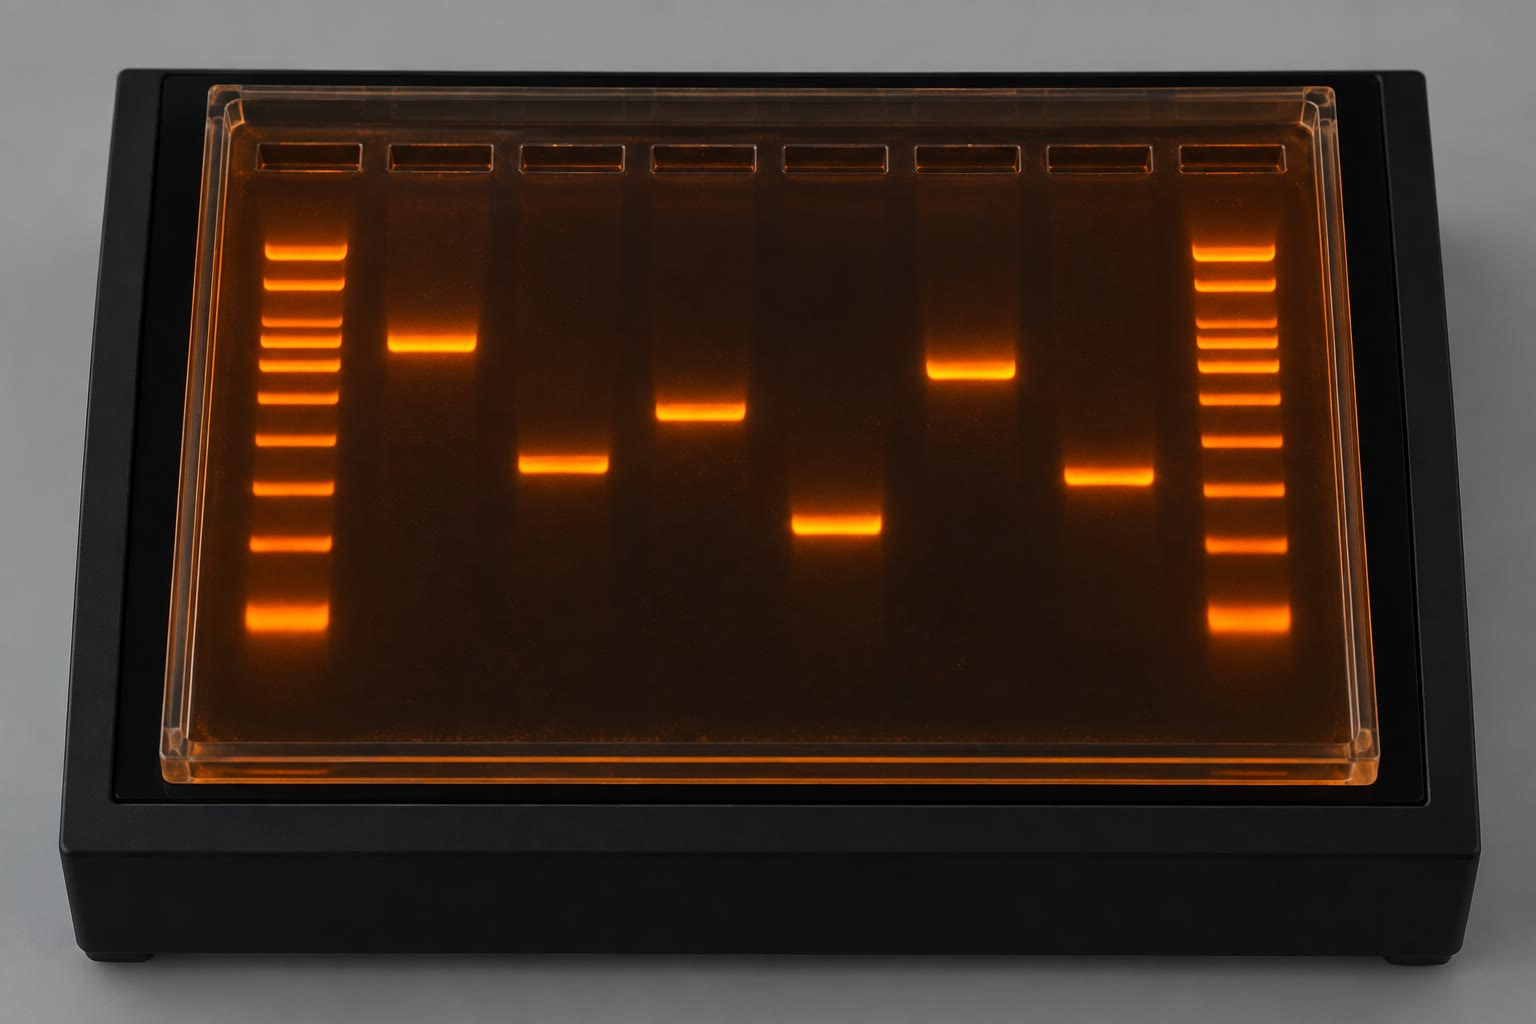
\includegraphics[width=0.56\linewidth]{images/book5/ai/b5-06-agarose-gel.jpg}

{\small Een agarosegel onder ultraviolet licht: DNA-fragmenten lopen
naar de anode met een snelheid die met hun lengte afneemt, zodat elke
band een populatie moleculen van één grootte is, vergeleken met de
ladder van bekende groottes in de buitenste banen.}
\end{omfigure}

\begin{definition}[De polymerasekettingreactie]\label{def:b3:genetic-engineering:pcr}
\index{polymerasekettingreactie}\index{primer}\index{kwantitatieve PCR}
De \emph{polymerasekettingreactie} (PCR) vermeerdert een gekozen stuk
DNA tussen twee \emph{primers} --- synthetische oligonucleotiden van
ongeveer twintig basen, complementair aan de twee strengen aan de
uiteinden van het doelwit --- via cycli van drie temperaturen:
\qty{95}{\celsius} om de strengen te scheiden,
\qtyrange{50}{65}{\celsius} om de primers te laten paren, en
\qty{72}{\celsius} om een hittebestendig polymerase (Taq, uit de
heetwaterbronbacterie \emph{Thermus aquaticus}) ze te laten verlengen.
Elke cyclus verdubbelt het aantal kopieën van het segment tussen de
primers, zodat dertig cycli van één molecuul een miljard maken. De
\emph{reverse-transcriptie-PCR} kopieert eerst RNA naar DNA en meet zo
transcripten of RNA-virussen; de \emph{kwantitatieve PCR} (qPCR) volgt
de vermeerdering in reële tijd met een fluorescerende kleurstof en
leest de beginhoeveelheid af uit de cyclus waarin het signaal een
drempel overschrijdt.
\end{definition}

\begin{theorem}[De rekenkunde van de vermeerdering]\label{thm:b3:genetic-engineering:pcr}
\index{drempelcyclus}
Bij een doeltreffendheid $E$ per cyclus ($E = 1$ voor volmaakte
verdubbeling) worden $N_{0}$ beginkopieën
\[
N_{n} = N_{0}\,(1 + E)^{n}
\]
na $n$ cycli. Overschrijdt de fluorescentie een vaste drempel wanneer
het aantal kopieën $N_{T}$ bereikt, dan is de \emph{\omterm{thm:b3:genetic-engineering:pcr}{drempelcyclus}}
\[
C_{T} = \frac{\log N_{T} - \log N_{0}}{\log(1 + E)},
\]
een rechte lijn in $\log N_{0}$ met richtingscoëfficiënt
$-1/\log(1+E)$: bij $E = 1$ verlaagt elke tienvoudige toename van de
beginhoeveelheid $C_{T}$ met $\log_{2} 10 = 3.32$ cycli, en twee
monsters waarvan de drempelcycli $\Delta C_{T}$ schelen verschillen in
beginkopieën met de factor $(1 + E)^{\Delta C_{T}}$.
\end{theorem}
\begin{proof}
Elke cyclus vermenigvuldigt het aantal kopieën met $1 + E$, dus is
$N_{n}$ een meetkundige rij. Stelt men $N_{n} = N_{T}$ en lost men naar
$n$ op, dan volgt $C_{T}$; de richtingscoëfficiënt is de coëfficiënt
van $\log N_{0}$. Voor twee monsters geldt
$C_{T,1} - C_{T,2} = (\log N_{0,2} - \log N_{0,1})/\log(1+E)$, waaruit
$N_{0,2}/N_{0,1} = (1+E)^{\Delta C_{T}}$.
\end{proof}

\begin{example}[Een qPCR-plaat lezen]\label{ex:b3:genetic-engineering:qpcr}
Een test op viraal RNA overschrijdt de drempel bij cyclus $22$ voor de
ene patiënt en bij cyclus $32$ voor de andere; bij $E \approx 1$ draagt
de eerste $2^{10}
\approx 1000$ keer zoveel virus. Een monster van tien kopieën
overschrijdt de drempel rond cyclus $37$ wanneer de drempel $10^{12}$
kopieën is ($\log_{2} 10^{11} =
36.5$); een run van $40$ cycli spoort dus enkele moleculen op, en één
enkel verontreinigend molecuul van een eerder product doet dat ook, en
daarom scheiden laboratoria de ruimtes waar PCR wordt opgezet van die
waar producten worden gehanteerd.
\end{example}

\begin{omfigure}
\begin{tikzpicture}
\begin{axis}[
  width=0.7\linewidth, height=5.6cm,
  axis x line=bottom, axis y line=left,
  xmin=0, xmax=40, ymin=1, ymax=1e14, ymode=log,
  xlabel={cyclus}, ylabel={kopieën},
  xlabel style={font=\small, at={(axis description cs:0.5,-0.12)}, anchor=north},
  ylabel style={font=\small},
  tick label style={font=\small}, xtick={0,10,20,30,40},
  clip=false,
]
\addplot[very thick, omDef, domain=0:40, samples=41] {1e7*2^x/(1+2^x/1e5)};
\addplot[very thick, omThm, domain=0:40, samples=41] {1e4*2^x/(1+2^x/1e8)};
\addplot[very thick, omMeth!70!black, domain=0:40, samples=41] {10*2^x/(1+2^x/1e11)};
\addplot[dashed, gray, domain=0:40, samples=2] {1e12};
\node[font=\scriptsize, gray, anchor=south west] at (axis cs:0.5,1.3e12) {drempel $N_{T}$};
\draw[gray] (axis cs:16.6,1) -- (axis cs:16.6,1e12); \draw[gray] (axis cs:26.6,1) -- (axis cs:26.6,1e12); \draw[gray] (axis cs:36.5,1) -- (axis cs:36.5,1e12);
\node[font=\scriptsize, anchor=south] at (axis cs:16.6,3e12) {$C_{T} = 16.6$}; \node[font=\scriptsize, anchor=south] at (axis cs:26.6,3e12) {$26.6$}; \node[font=\scriptsize, anchor=south] at (axis cs:36.5,3e12) {$36.5$};
\end{axis}
\end{tikzpicture}

{\small Vermeerderingscurven voor $N_{0} = 10^{7}$ (blauw), $10^{4}$
(rood) en $10$ kopieën (groen), $E = 1$, met het plateau dat de
reagentia opleggen. Een duizendvoudig verschil in $N_{0}$ verschuift de
\omterm{thm:b3:genetic-engineering:pcr}{drempelcyclus} met $10$; de plateaus zijn alle gelijk, en daarom zegt
het eindproduct niets over het begin.}
\end{omfigure}

\section{Eiwitten maken}

\begin{definition}[Expressiesystemen]\label{def:b3:genetic-engineering:expression}
\index{expressievector}\index{recombinant eiwit}\index{monoklonaal antilichaam}
Een \emph{expressievector} plaatst de gekloneerde coderende sequentie
onder een sterke, regelbare promotor van de gastheer (de \emph{lac}- of
T7-promotor in \emph{E.~coli}, aangezet met een suikeranaloog), met een
ribosoombindingsplaats, een terminator en vaak een \emph{tag} --- zes
histidines, een klein eiwit --- die aan het product wordt gefuseerd om
het over een kolom te zuiveren. Bacteriën maken grammen per liter van
een eenvoudig eiwit (insuline, groeihormoon, enzymen) maar kunnen
complexe zoogdiereiwitten niet glycosyleren of vouwen; gist voegt
suikers van eigen soort toe; insecten- en zoogdiercellen
(ovariumcellen van de Chinese hamster zijn de norm in de industrie)
maken antilichamen en stollingsfactoren die zijn gevouwen en
geglycosyleerd als bij de mens. Een \emph{monoklonaal antilichaam}
wordt gemaakt door een \emph{hybridoom} --- een antilichaamproducerende
B-cel gefuseerd met een onsterfelijke myeloomcel (Köhler en Milstein,
1975) --- of tegenwoordig door de antilichaamgenen in een
zoogdierexpressielijn te kloneren, waar het muizenraamwerk door
menselijke sequentie kan worden vervangen om afstoting te vermijden
(\cref{ch:b3:adaptive-immunity}).
\end{definition}

\begin{example}[Insuline]\label{ex:b3:genetic-engineering:insulin}
Menselijke insuline bestaat uit twee ketens, A (21 residuen) en B (30),
verbonden door zwavelbruggen en in de $\beta$-cel uit één enkele
voorloper, pro-insuline, geknipt. Het eerste proces bracht de twee
ketens afzonderlijk in \emph{E.~coli} tot expressie, elk gefuseerd aan
$\beta$-galactosidase, knipte ze er chemisch af en voegde ze in vitro
samen; latere processen brengen pro-insuline tot expressie en knippen
het met de enzymen die de alvleesklier gebruikt. Sinds 1996 is ook de
sequentie zelf veranderd: één of twee residuen verwisselen of
toevoegen geeft analogen die sneller uiteenvallen (voor bij een
maaltijd) of op de injectieplaats neerslaan en over een dag vrijkomen.
Een eiwit dat acht ton klieren per kilogram kostte wordt nu in een
fermentor gemaakt, gelijk aan het menselijke of beter dan dat.
\end{example}

\section{Transgene organismen}

\begin{definition}[Transgenese en gerichte genmodificatie]\label{def:b3:genetic-engineering:transgenic}
\index{transgeen organisme}\index{micro-injectie}\index{knock-out}\index{embryonale stamcel}\index{gerichte genmodificatie}
Een \emph{transgeen} organisme draagt een gen dat in zijn kiembaan is
ingebracht, zodat elke cel het heeft en het wordt geërfd. Bij muizen is
de klassieke weg de \emph{micro-injectie} van het DNA in één voorkern
van een bevruchte eicel (Gordon en Ruddle, 1980), waarna het bij een
deel van de embryo's op een willekeurige plaats integreert; Palmiter en
Brinster (1982) maakten muizen van tweemaal de normale grootte door het
rattengen voor groeihormoon achter een metallothioneïnepromotor in te
spuiten. De \emph{gerichte genmodificatie} vervangt of verstoort in
plaats daarvan een gekozen gen: een construct met lange armen die
homoloog zijn aan het doelwit wordt in \emph{embryonale stamcellen}
gebracht, de zeldzame cellen waarin de \omterm{def:b3:dna-repair:dsb}{homologe recombinatie} het op de
juiste plaats heeft gezet worden geselecteerd en in een blastocyst
gespoten, en de chimere muis die daaruit ontstaat geeft het gewijzigde
gen door (Capecchi, Smithies en Evans, jaren tachtig). Een
\emph{knock-out} mist het gen; een \emph{knock-in} draagt een gewijzigde
versie; een \emph{conditioneel} allel, geflankeerd door loxP-plaatsen,
wordt alleen verwijderd waar en wanneer Cre tot expressie komt
(\cref{ch:b3:dna-repair}). Zo'n tienduizend muizengenen zijn
uitgeschakeld, en voor de meeste was het fenotype de eerste aanwijzing
van wat het gen doet.
\end{definition}

\begin{omfigure}
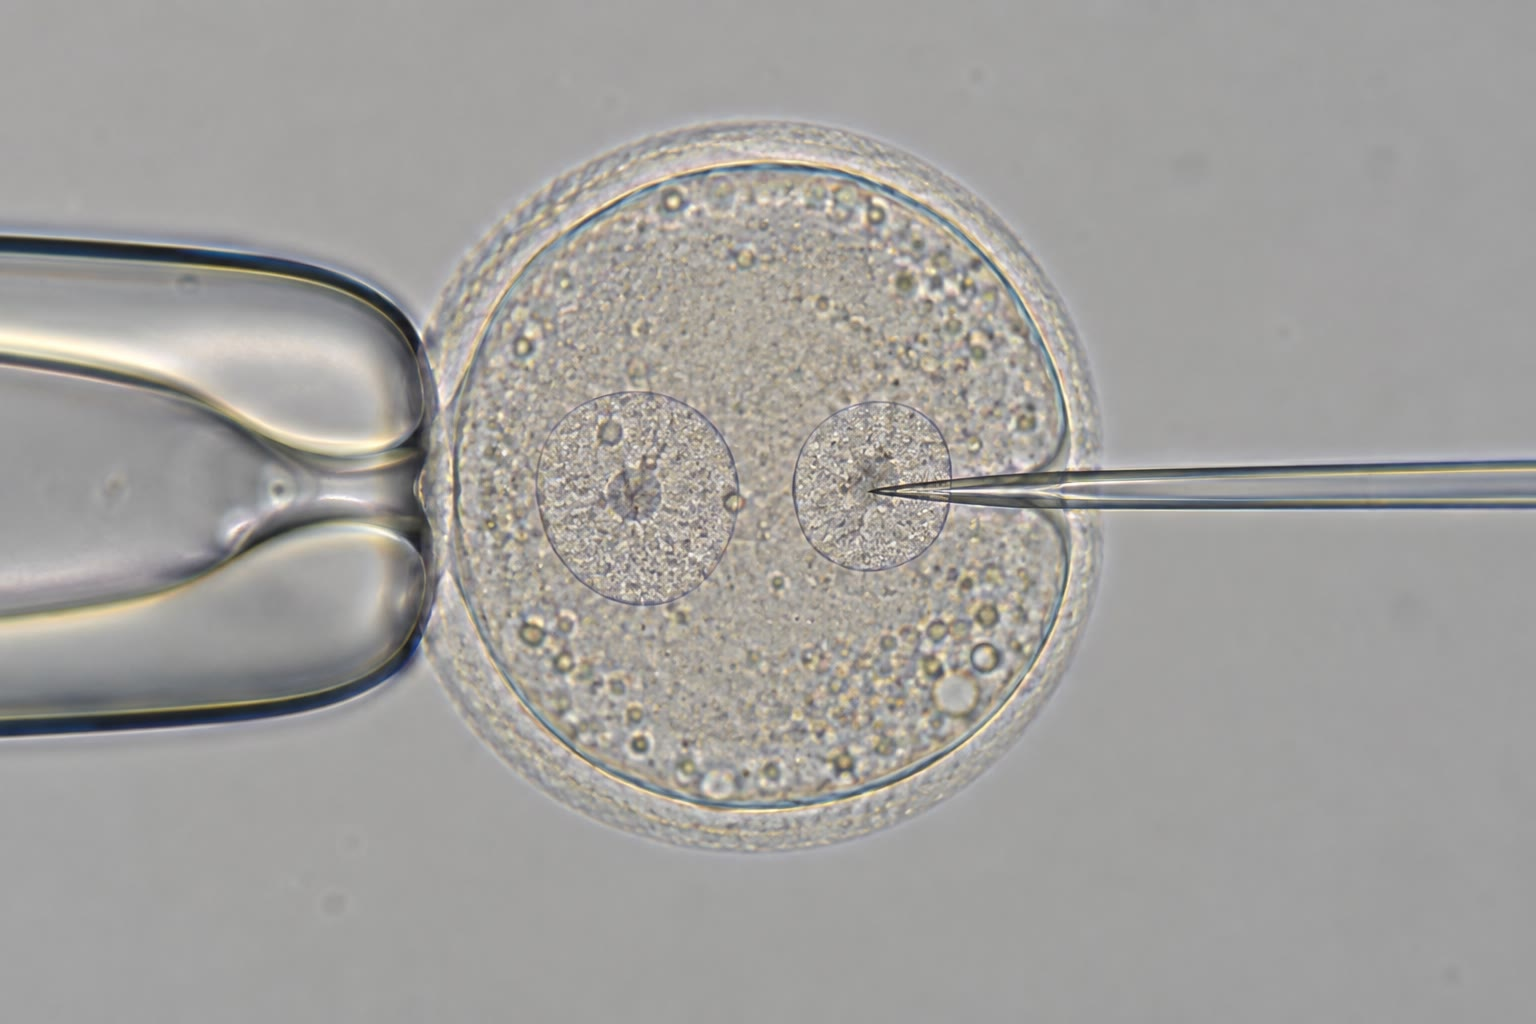
\includegraphics[width=0.46\linewidth]{images/book5/ai/b5-06-microinjection.jpg}\hspace{0.04\linewidth}
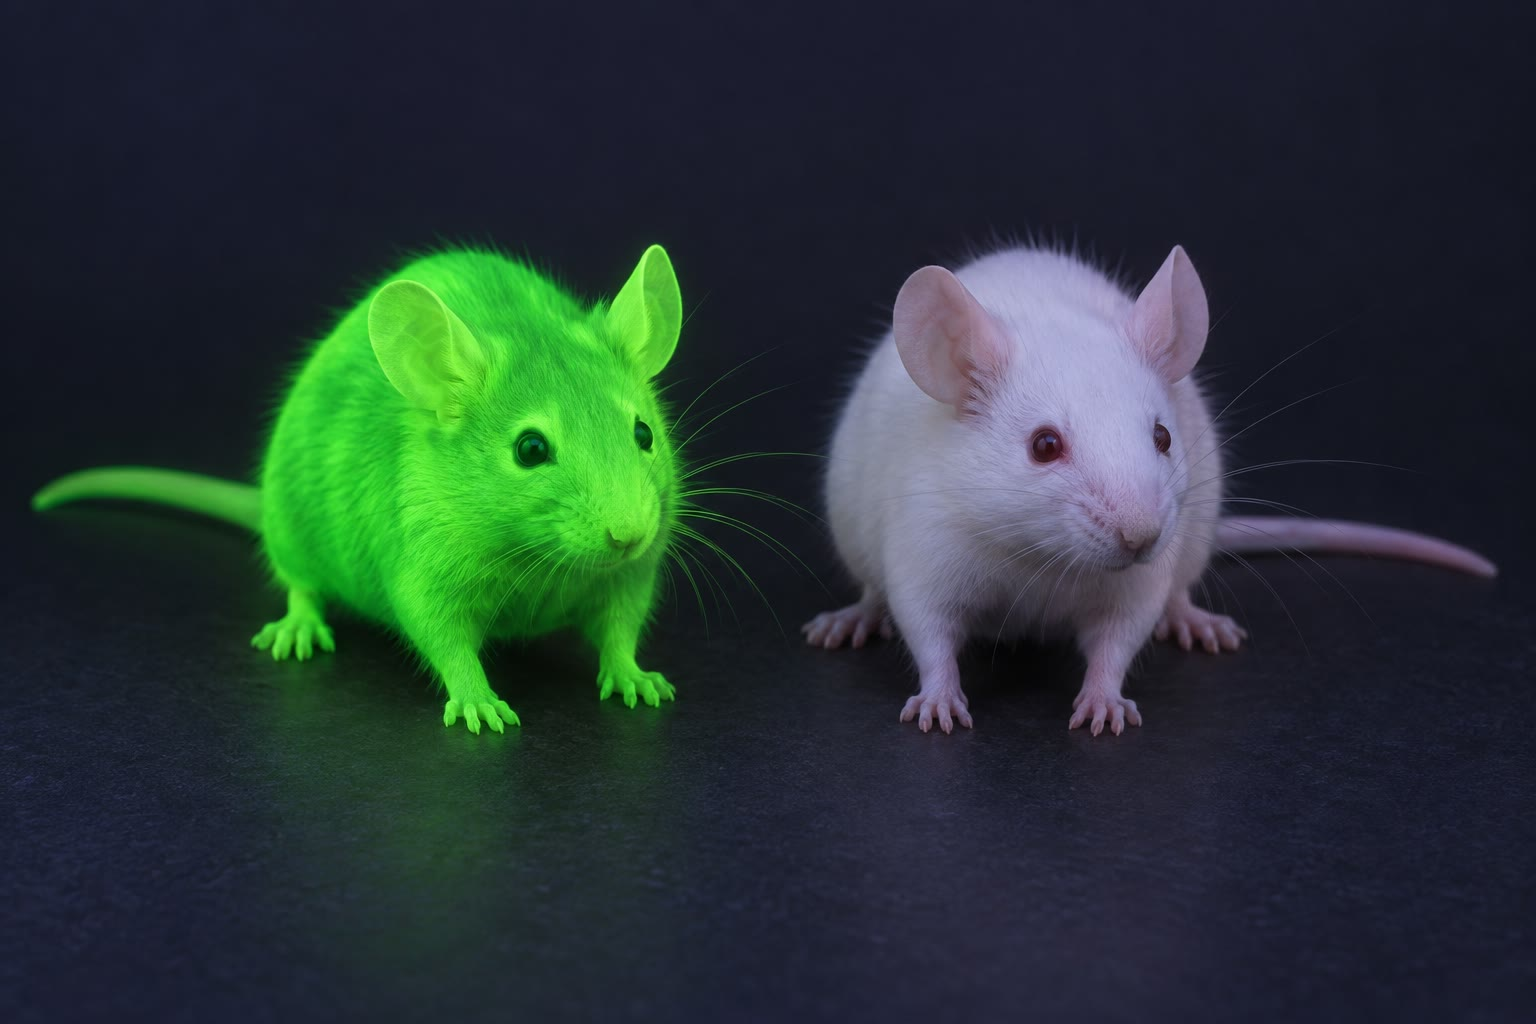
\includegraphics[width=0.46\linewidth]{images/book5/ai/b5-06-gfp-mouse.jpg}

{\small Links: een bevruchte muizeneicel die door zuiging wordt
vastgehouden terwijl een glazen naald DNA in één voorkern spuit.
Rechts: een transgene muis die het groene fluorescerende eiwit van een
kwal in elke cel tot expressie brengt, naast een gewone nestgenoot,
onder ultraviolet licht.}
\end{omfigure}

\begin{definition}[Transgene planten]\label{def:b3:genetic-engineering:plants}
\index{Agrobacterium}\index{T-DNA}\index{genetisch gemodificeerd gewas}
Planten worden getransformeerd met \emph{Agrobacterium tumefaciens},
een bodembacterie die van nature een deel van haar tumorinducerende
\omterm{def:b3:genetic-engineering:tools}{plasmide}, het \emph{T-DNA}, in het genoom van een gewonde plant invoegt
om die een gal te laten vormen die de bacterie voedt. De eigen genen
van het T-DNA vervangen door een willekeurig gen, tussen de
grenssequenties die de bacterie herkent, maakt van de ziekteverwekker
een \omterm{def:b3:genetic-engineering:tools}{vector}; de getransformeerde cellen worden geselecteerd en tot hele
planten geregenereerd, wat elke plantencel kan. Soorten die de bacterie
niet infecteert (lange tijd de granen) worden getransformeerd door met
DNA beklede gouddeeltjes in weefsel te schieten. \emph{Genetisch
gemodificeerde gewassen} die op grote schaal worden geteeld dragen een
bacterieel toxinegen (\emph{Bt}) tegen insectenlarven, of een bacterieel
enzym dat verdraagzaamheid voor een onkruidbestrijder geeft, of beide;
\emph{Golden Rice} draagt twee genen van de carotenoïdroute (een
plantaardig fytoeensynthase en een bacterieel desaturase) zodat zijn
endosperm $\beta$-caroteen maakt, de voorloper van vitamine~A, waarvan
het tekort jaarlijks enkele honderdduizenden kinderen blind maakt en
doodt.
\end{definition}

\begin{omfigure}
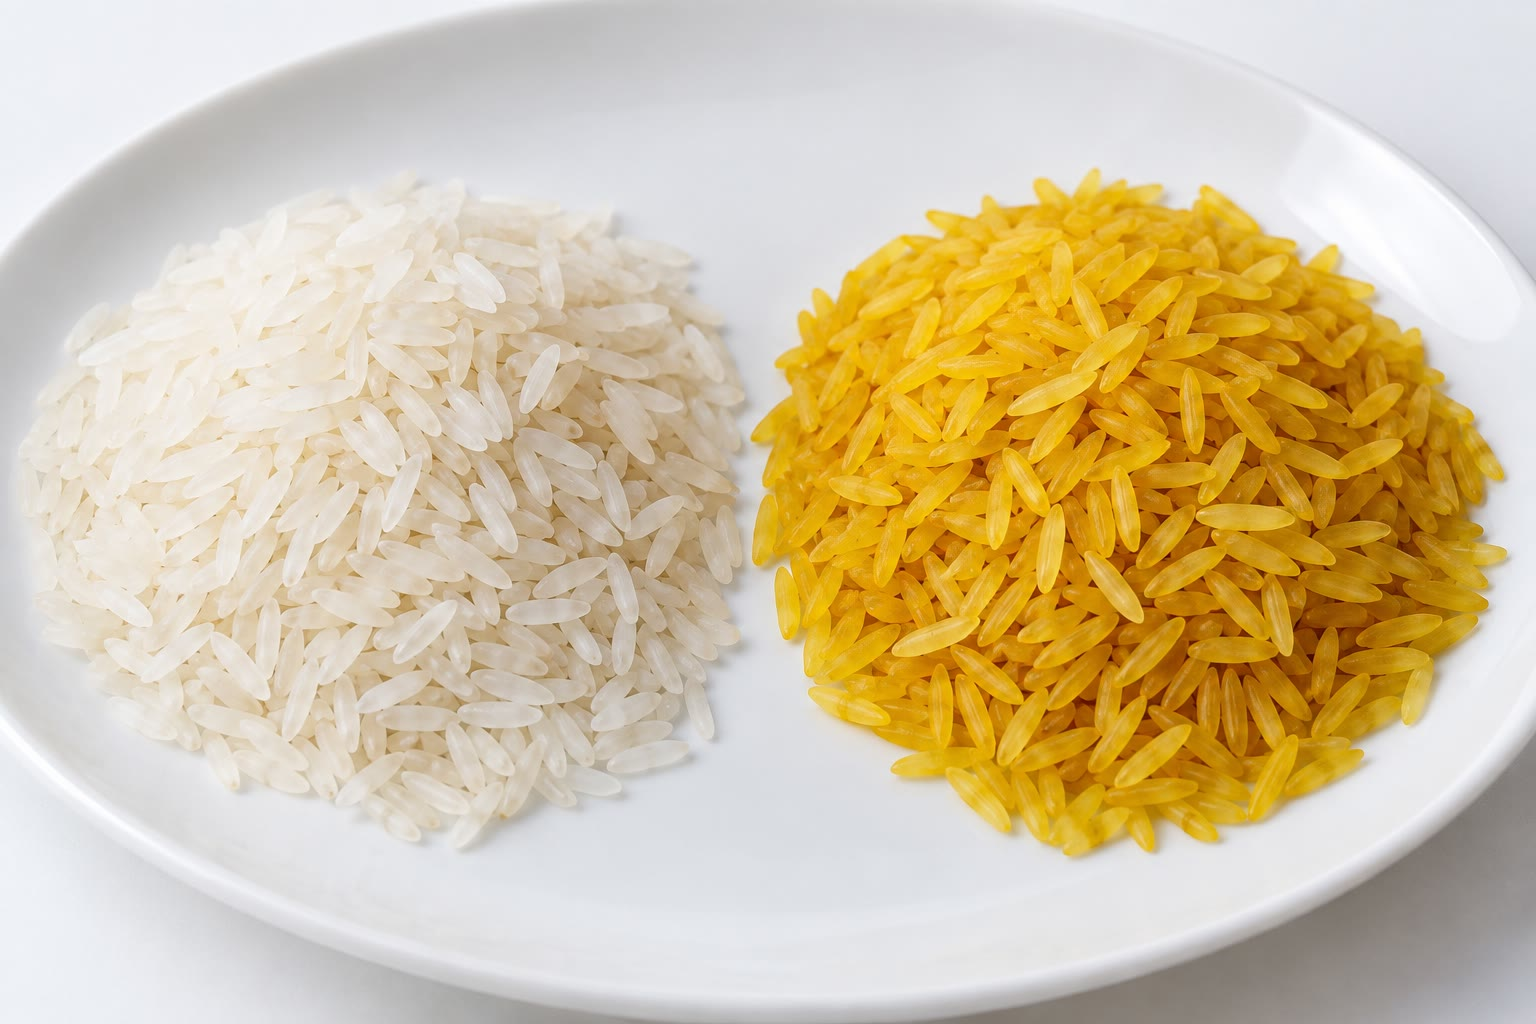
\includegraphics[width=0.46\linewidth]{images/book5/ai/b5-06-golden-rice.jpg}\hspace{0.04\linewidth}
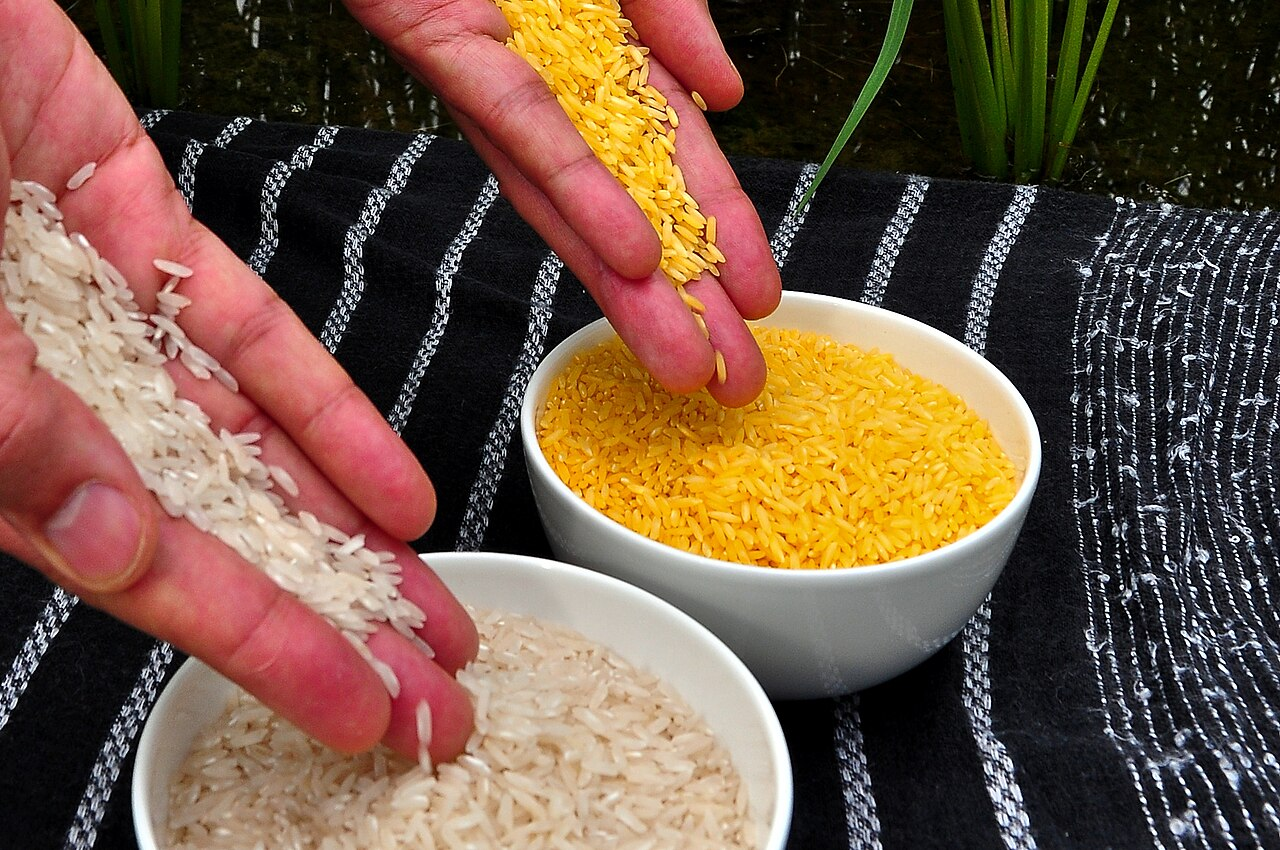
\includegraphics[width=0.46\linewidth]{images/book5/golden-rice-irri.jpg}

{\small Gewone rijst en Golden Rice. De gele korrel maakt in haar
endosperm $\beta$-caroteen uit twee toegevoegde genen van de
carotenoïdroute. Rechts: de twee rijstsoorten vergeleken bij het
International Rice Research Institute (IRRI, CC~BY~2.0).}
\end{omfigure}

\begin{remark}[Het debat]\label{rem:b3:genetic-engineering:gmo}
Dertig jaar teelt op honderden miljoenen hectaren, en elke
stelselmatige beoordeling door wetenschappelijke academies, hebben geen
enkel gezondheidseffect van goedgekeurde transgene gewassen gevonden
dat van dat van hun gewone tegenhangers verschilt; het transgen is één
gen te midden van veertigduizend, en het eiwit dat het maakt wordt
getoetst zoals elk levensmiddelenadditief. De werkelijke vragen zijn
ecologisch en economisch: de verspreiding van resistentie bij plagen en
onkruiden onder eenvormige selectie, genenstroom naar wilde verwanten,
de concentratie van de zaadmarkt, en wie ervan profiteert. Het zijn de
vragen die elke krachtige landbouwtechniek oproept, en de antwoorden
hangen af van de eigenschap en van de omstandigheden, niet van de
methode waarmee het gen is verplaatst.
\end{remark}

\section{Genomen bewerken}

\begin{definition}[CRISPR--Cas9]\label{def:b3:genetic-engineering:crispr}
\index{CRISPR}\index{Cas9}\index{gids-RNA}\index{PAM}\index{genoombewerking}
Bacteriën bewaren fragmenten van de genomen van fagen die hun
voorouders hebben besmet in een reeks herhalingen (\emph{CRISPR}),
schrijven ze af tot korte gids-RNA's, en sturen daarmee een nuclease
naar elk passend DNA dat de cel binnenkomt: een adaptief afweersysteem
met een genetisch geheugen. Bij \emph{Streptococcus pyogenes} is het
nuclease het enkele eiwit \emph{Cas9}, dat een gids-RNA en een tweede
klein RNA bindt, DNA afzoekt op een \emph{protospacer-aangrenzend
\omterm{def:b3:bioinformatics:motif}{motief}} van drie basen (PAM, 5$'$-NGG), het aangrenzende DNA ontwindt
en, als de twintig basen naast de PAM met de gids paren, beide strengen
drie basen van de PAM doorknipt. Jinek, Charpentier, Doudna en
collega's (2012) versmolten de twee RNA's tot één \emph{enkelvoudig
gids-RNA} en toonden aan dat Cas9 met een gids van willekeurige
sequentie DNA op die sequentie in een reageerbuis knipt; binnen een
jaar was aangetoond dat het paar werkt in cellen van mens, muis,
zebravis, plant en gist. \emph{Genoombewerking} is wat de cel met de
knip doet: eindverbinding laat een kleine insertie of deletie achter
die het gen verstoort (een \omterm{def:b3:genetic-engineering:transgenic}{knock-out} in één stap, in elk organisme,
binnen weken), en \omterm{def:b3:dna-repair:dsb}{homologe recombinatie} met een aangeboden matrijs
schrijft er een gekozen sequentie in.
\end{definition}

\begin{omfigure}
\begin{tikzpicture}[every node/.style={font=\scriptsize}, >=stealth]
  % Cas9 outline (drawn first so labels stay on top)
  \draw[thick, omExo, fill=omExo!15] (5.9,1.1) ellipse (2.6 and 1.6);
  \node[omExo!60!black] at (7.7,2.3) {Cas9};
  % target DNA
  \draw[very thick, omDef] (0,0.3) -- (11,0.3); \draw[very thick, omDef] (0,-0.1) -- (11,-0.1);
  % PAM
  \fill[omProp!60] (7.2,-0.2) rectangle (7.9,0.4); \node[below] at (7.55,-0.25) {PAM (NGG)};
  % protospacer
  \draw[omThm, very thick] (4.2,0.5) -- (7.15,0.5); \node[above] at (5.7,0.55) {doelwit van 20 basen, gepaard met de gids};
  % guide RNA
  \draw[very thick, omMeth!70!black] (4.2,0.3) .. controls (4.2,1.6) and (5.0,1.9) .. (5.4,1.9) -- (6.6,1.9) .. controls (7.0,1.9) and (7.2,2.5) .. (6.8,2.8) .. controls (6.3,3.1) and (5.8,2.7) .. (6.1,2.4);
  \node[left, omMeth!70!black, align=right] at (3.2,2.2) {enkelvoudig gids-RNA:\\20 basen naar keuze\\+ haarspeld die Cas9 bindt};
  % cut
  \draw[omThm, very thick, ->] (6.25,-0.7) -- (6.25,0.35); \node[omThm, below] at (6.25,-0.7) {dubbelstrengsbreuk, 3 basen van de PAM};
  % outcomes
  \draw[->, thick] (2.0,-1.3) -- (2.0,-1.9); \node[below, align=center] at (2.0,-1.9) {eindverbinding:\\kleine insertie of deletie\\$\Rightarrow$ leesraamverschuiving, knock-out};
  \draw[->, thick] (10.0,-1.3) -- (10.0,-1.9); \node[below, align=center] at (10.0,-1.9) {recombinatie met een\\aangeboden matrijs\\$\Rightarrow$ nauwkeurige verandering};
\end{tikzpicture}

{\small \omterm{def:b3:genetic-engineering:crispr}{Cas9} en zijn gids. Het eiwit bindt een \omterm{def:b3:genetic-engineering:crispr}{PAM}, ontwindt het DNA
ernaast, en knipt als de twintig basen met het \omterm{def:b3:genetic-engineering:crispr}{gids-RNA} paren. De breuk
wordt hersteld ofwel door eindverbinding, die het gen verstoort, ofwel
door recombinatie met een matrijs, die het herschrijft.}
\end{omfigure}

\begin{proposition}[Bewerken zonder breuk]\label{prop:b3:genetic-engineering:editors}
\index{basebewerker}\index{prime-bewerker}\index{off-target}
Beide strengen doorknippen is de grofste bewerking: de uitkomst van de
eindverbinding is willekeurig, en een breuk elders --- een
\emph{off-target}-plaats die op enkele posities van de gids afwijkt en
die \omterm{def:b3:genetic-engineering:crispr}{Cas9} duldt --- is een mutatie waar niemand om vroeg. Een \omterm{def:b3:genetic-engineering:crispr}{Cas9}
waarvan één nucleasedomein is uitgeschakeld knipt één streng in; met
beide uitgeschakeld bindt het alleen nog, en kan het andere enzymen
naar een sequentie brengen. \emph{\omterm{prop:b3:genetic-engineering:editors}{Basebewerkers}} fuseren een inknippend
\omterm{def:b3:genetic-engineering:crispr}{Cas9} aan een deaminase dat in de ontwonden streng C naar U omzet
(gelezen als T) of A naar I (gelezen als G), en veranderen zo één base
zonder breuk en zonder matrijs; \emph{\omterm{prop:b3:genetic-engineering:editors}{prime-bewerkers}} dragen een
reverse transcriptase en een gids die met de gewenste sequentie is
verlengd, en kopiëren die sequentie in de ingeknipte streng, wat elke
substitutie en kleine inserties of deleties toelaat. Activiteit buiten
het doelwit wordt beperkt door Cas9-varianten met hoge getrouwheid, door
het enzym kortstondig als eiwit in plaats van als gen aan te bieden, en
door gidsen te kiezen waarvan de naaste genomische verwanten op
verscheidene posities verschillen; zij wordt gemeten door de voorspelde
plaatsen te sequencen en met onbevooroordeelde methoden die elke breuk
in het genoom vangen.
\end{proposition}

\begin{example}[Een genezing]\label{ex:b3:genetic-engineering:sickle}
Sikkelcelziekte is één basenverandering in $\beta$-globine. Foetaal
hemoglobine, gemaakt uit $\gamma$-globine, zou het kunnen vervangen,
maar de $\gamma$-genen worden na de geboorte uitgezet door de repressor
BCL11A. De eerste goedgekeurde CRISPR-therapie (2023) neemt de eigen
bloedstamcellen van de patiënt, knipt met \omterm{def:b3:genetic-engineering:crispr}{Cas9} de erytroïde enhancer
van \emph{BCL11A} door zodat de eindverbinding haar in de meeste cellen
uitschakelt, en geeft de cellen terug nadat het beenmerg van de patiënt
is leeggemaakt: de rode cellen die zij maken zijn rijk aan foetaal
hemoglobine, sikkelen niet, en de crises houden op. De bewerking is
somatisch --- de kiembaan blijft onaangeroerd en de verandering wordt
niet geërfd --- en zij gebruikt de ``grove'' uitkomst, verstoring,
juist waar verstoring is wat men wil.
\end{example}

\begin{theorem}[Supermendeliaanse verspreiding van een gendrive]\label{thm:b3:genetic-engineering:drive}
\index{gendrive}
Een \emph{\omterm{thm:b3:genetic-engineering:drive}{gendrive}} is een construct dat codeert voor \omterm{def:b3:genetic-engineering:crispr}{Cas9} en een gids
die in een heterozygoot het wildtype-allel op zijn eigen locus knipt;
herstel door recombinatie kopieert de drive in het geknipte chromosoom,
zodat een deel $c$ van de gameten van de heterozygoot de drive draagt
in plaats van de mendeliaanse helft. Heeft de drive frequentie $p$ in
een grote, willekeurig parende populatie en geen fitnesskosten, dan is
haar frequentie in de volgende generatie
\[
p' = p + c\,p\,(1 - p),
\]
zodat zij zich vanuit zeldzaamheid verspreidt met een snelheid
evenredig aan $c$, en de helft van de populatie bereikt in ongeveer
$\ln(1/p_{0})/\ln(1 + c)$ generaties vanaf een beginfrequentie $p_{0}$.
\end{theorem}
\begin{proof}
Willekeurige paring geeft homozygoten voor de drive met frequentie
$p^{2}$, heterozygoten met $2p(1-p)$ en wildtype-homozygoten met
$(1-p)^{2}$. De homozygoten geven de drive aan al hun gameten door, de
heterozygoten aan een deel $(1 + c)/2$ (de helft volgens Mendel, plus
$c$ maal de omgezette wildtypehelft), de wildtypes aan geen enkele.
Dus $p' = p^{2} + 2p(1-p)(1+c)/2
= p^{2} + p(1-p) + c\,p(1-p) = p + c\,p(1-p)$. Voor kleine $p$ is dit
$p' \approx (1+c)p$, meetkundige groei met verhouding $1 + c$, die
$1/2$ bereikt vanaf $p_{0}$ na ongeveer $\ln(1/2p_{0})/\ln(1+c)$
generaties; de logistische term remt haar pas tegen het eind.
\end{proof}

\begin{omfigure}
\begin{tikzpicture}
\begin{axis}[
  width=0.7\linewidth, height=5.6cm,
  axis x line=bottom, axis y line=left,
  xmin=0, xmax=20, ymin=0, ymax=1.05,
  xlabel={generatie}, ylabel={frequentie $p$ van de drive},
  xlabel style={font=\small, at={(axis description cs:0.5,-0.12)}, anchor=north},
  ylabel style={font=\small},
  tick label style={font=\small}, xtick={0,5,10,15,20}, ytick={0,0.5,1},
  clip=false,
]
\addplot[very thick, omThm, mark=*, mark size=1.2pt] coordinates {(0,0.01) (1,0.0189) (2,0.0356) (3,0.0665) (4,0.1224) (5,0.2191) (6,0.3731) (7,0.5836) (8,0.8023) (9,0.9451) (10,0.9918) (11,0.9991) (12,1.0) (13,1.0) (14,1.0) (15,1.0) (16,1.0) (17,1.0) (18,1.0) (19,1.0) (20,1.0)};
\addplot[very thick, omDef, mark=*, mark size=1.2pt] coordinates {(0,0.01) (1,0.015) (2,0.0223) (3,0.0332) (4,0.0493) (5,0.0727) (6,0.1064) (7,0.154) (8,0.2191) (9,0.3047) (10,0.4106) (11,0.5316) (12,0.6561) (13,0.769) (14,0.8578) (15,0.9188) (16,0.9561) (17,0.9771) (18,0.9883) (19,0.9941) (20,0.997)};
\addplot[very thick, gray, dashed, domain=0:20, samples=2] {0.01};
\node[font=\scriptsize, omThm, anchor=south east] at (axis cs:6.5,0.62) {$c = 0.9$};
\node[font=\scriptsize, omDef, anchor=north west] at (axis cs:12.5,0.62) {$c = 0.5$};
\node[font=\scriptsize, gray, anchor=south west] at (axis cs:12,0.02) {mendeliaans, $c = 0$: blijft op $p_{0}$};
\end{axis}
\end{tikzpicture}

{\small Een \omterm{thm:b3:genetic-engineering:drive}{gendrive} losgelaten bij één procent, met een
omzettingsdoeltreffendheid van $0.9$ of $0.5$ en zonder fitnesskosten.
Een mendeliaans allel zonder voordeel zou op één procent blijven; de
drive neemt het in tien of twintig generaties over.}
\end{omfigure}

\begin{remark}[Wat bewerkt mag worden]\label{rem:b3:genetic-engineering:ethics}
De somatische cellen van een instemmende patiënt bewerken is
geneeskunde, te beoordelen als elke behandeling naar risico's en baten.
De kiembaan bewerken --- een embryo, waarvan elke afstammeling de
verandering zou dragen --- is van een andere orde: de betrokken persoon
kan niet instemmen, de verandering wordt geërfd, en de uitkomsten
buiten het doelwit en in mozaïek zijn nog niet beheerst; nadat een
Chinese onderzoeker in 2018 bekendmaakte dat hij het bij een tweeling
had gedaan, riepen de wetenschappelijke academies van de meeste landen
op tot een moratorium en maakten verscheidene staten het strafbaar. Een
\omterm{thm:b3:genetic-engineering:drive}{gendrive} die in een wilde populatie wordt losgelaten is een beslissing
die voor iedereen stroomafwaarts wordt genomen, en daarom koppelt het
vakgebied in zijn eigen voorstellen om malariamuggen uit te roeien de
drives aan noodremmen --- omkeerdrives, zelfbeperkende ontwerpen --- en
aan publieke instemming in de betrokken landen.
\end{remark}

\section{Opgaven}

\begin{exercise}[$\star$]\label{exo:b3:genetic-engineering:1}
Noem de drie onderdelen die een kloneringsplasmide moet hebben en leg
het doel van elk uit.
\end{exercise}

\begin{exercise}[$\star$]\label{exo:b3:genetic-engineering:2}
EcoRI herkent GAATTC. Hoe vaak komt de plaats gemiddeld voor in
willekeurig DNA, en hoeveel fragmenten maakt zij van het genoom van
\emph{E.~coli} van \qty{4.6}{Mb}? Waarom is het werkelijke aantal
enigszins anders?
\end{exercise}

\begin{exercise}[$\star$]\label{exo:b3:genetic-engineering:3}
Noem de drie temperatuurstappen van een PCR-cyclus en wat er bij elk
gebeurt. Waarom moet het polymerase hittebestendig zijn?
\end{exercise}

\begin{exercise}[$\star$]\label{exo:b3:genetic-engineering:4}
Wat heeft \omterm{def:b3:genetic-engineering:crispr}{Cas9} nodig om een gegeven sequentie te knippen, en welke twee
uitkomsten kunnen op de knip volgen?
\end{exercise}

\begin{exercise}[$\star\star$]\label{exo:b3:genetic-engineering:5}
Een PCR loopt $35$ cycli bij doeltreffendheid $E = 0.9$ vanaf $50$
kopieën. Hoeveel kopieën levert dat op? Een qPCR van twee monsters
geeft $C_{T} = 18.2$ en $25.5$; wat is bij $E = 0.95$ de verhouding van
hun beginhoeveelheden?
\end{exercise}

\begin{exercise}[$\star\star$]\label{exo:b3:genetic-engineering:6}
Waarom wordt voor de expressie van een menselijk eiwit in bacteriën een
cDNA-bibliotheek gebruikt en geen genomische bibliotheek? Noem twee
andere hindernissen bij het maken van een menselijk eiwit in
\emph{E.~coli} en zeg hoe elk wordt genomen.
\end{exercise}

\begin{exercise}[$\star\star$]\label{exo:b3:genetic-engineering:7}
Een knock-outmuis wordt gemaakt met \omterm{def:b3:genetic-engineering:transgenic}{gerichte genmodificatie} in
embryonale stamcellen. Leg uit waarom de eerste muis die wordt geboren
een chimeer is, waarom men haar moet doorfokken, en welk deel van de
kleinkinderen van een chimeer waarvan de kiembaan half gemodificeerd is
homozygoot \omterm{def:b3:genetic-engineering:transgenic}{knock-out} is als heterozygote grootouders onderling worden
gekruist.
\end{exercise}

\begin{exercise}[$\star\star$]\label{exo:b3:genetic-engineering:8}
Er wordt een \omterm{def:b3:genetic-engineering:crispr}{gids-RNA} van 20 basen met een \omterm{def:b3:genetic-engineering:crispr}{NGG-PAM} gekozen. Hoeveel
plaatsen in een genoom van $3.2\times 10^{9}$ bp (beide strengen) passen
door toeval precies op de gids? Hoeveel passen met hoogstens twee
verschillen, als \omterm{def:b3:genetic-engineering:crispr}{Cas9} die duldt? (Tel het aantal sequenties binnen twee
verschillen als $1 + 3\binom{20}{1} +
9\binom{20}{2}$.)
\end{exercise}

\begin{exercise}[$\star\star$]\label{exo:b3:genetic-engineering:9}
Bereken met \cref{thm:b3:genetic-engineering:drive} de frequentie van
een drive met $c = 0.8$ na drie generaties vanaf $p_{0} = 0.05$, en
schat het aantal generaties tot $0.5$.
\end{exercise}

\begin{exercise}[$\star\star\star$]\label{exo:b3:genetic-engineering:10}
De therapie voor sikkelcelziekte verstoort een enhancer in plaats van
de mutatie in $\beta$-globine te corrigeren. Geef twee redenen waarom
in bloedstamcellen voor verstoring door eindverbinding is gekozen en
niet voor correctie door \omterm{def:b3:dna-repair:dsb}{homologe recombinatie}, en één nadeel.
\end{exercise}

\begin{exercise}[$\star\star\star$]\label{exo:b3:genetic-engineering:11}
Een \omterm{thm:b3:genetic-engineering:drive}{gendrive} tegen een mug brengt bij homozygoten fitnesskosten $s$ met
zich mee. Pas de recursie aan zodat zij selectie tegen homozygoten voor
de drive omvat, en zoek de voorwaarde op $c$ en $s$ waaronder de drive
zich vanuit zeldzaamheid verspreidt. Leg daarna uit waarom
resistentie-allelen --- producten van de eindverbinding op het doelwit
die de gids niet meer herkent --- in de praktijk de voornaamste
hindernis zijn.
\end{exercise}

\begin{exercise}[$\star\star\star$]\label{exo:b3:genetic-engineering:12}
Beredeneer met de mechanismen van dit hoofdstuk en van
\cref{ch:b3:dna-repair} waarom het bewerken van de kiembaan van een
menselijk embryo op dit moment de beoogde uitkomst niet in elke cel kan
waarborgen, en welk bewijs nodig zou zijn voordat een redelijk mens het
veilig zou kunnen achten.
\end{exercise}

\section{Vraagstuk: van een gen naar een geneesmiddel en een gewas}

\begin{problem}[{Weekendvraagstuk --- een gen gekloneerd met de
rekenkunde van restrictieplaatsen en transformatie, een virus geteld
met qPCR, een hormoon per ton in een fermentor gemaakt, een genoom
bewerkt met telling van de treffers buiten het doelwit, en een gendrive
in de tijd gezet, met als besluit de kopieën van een virus in een
monster, het jaarlijkse fermentorvolume voor de insuline van de wereld
en het aantal generaties dat een drive nodig heeft}]
\label{pb:b3:genetic-engineering:1}
Gegevens: een gen van \qty{1.5}{kb}; een restrictieplaats van zes
basen; een \omterm{def:b3:genetic-engineering:tools}{plasmide} van \qty{4}{kb}; transformatiedoeltreffendheid
$2\times 10^{7}$ kolonies per microgram \omterm{def:b3:genetic-engineering:tools}{plasmide}; de ligatie geeft
\qty{10}{\%} van de \omterm{def:b3:genetic-engineering:tools}{plasmiden} een invoegsel.
qPCR-doeltreffendheid $E = 1$, drempel $N_{T} = 10^{12}$. Insuline:
\qty{5.8}{kDa}, een patiënt gebruikt $40$ eenheden per dag, en één
eenheid is \qty{35}{\micro g}; $10^{7}$ patiënten; een fermentor levert
\qty{2}{g/L} product per partij, tien partijen per jaar. Genoom
$3.2\times
10^{9}$ bp. Omzetting van de drive $c = 0.9$, losgelaten bij
$p_{0} = 0.001$.

\medskip
\noindent\textbf{Deel I --- Kloneren.}
\begin{enumerate}
  \item Hoe vaak komt een gegeven plaats van zes basen voor in
        willekeurig DNA? Wat is de kans dat het gen van \qty{1.5}{kb}
        geen zo'n plaats bevat, zodat het enzym kan worden gebruikt om
        het in zijn geheel te kloneren?
  \item Als het er wel een bevat, hoe zou het dan toch te kloneren
        zijn? (Twee methoden.)
  \item Er wordt \qty{100}{ng} geligeerd \omterm{def:b3:genetic-engineering:tools}{plasmide} getransformeerd.
        Hoeveel kolonies, en hoeveel daarvan dragen het invoegsel?
  \item Er wordt blauw-witscreening gebruikt. Welk deel van de kolonies
        is wit, en hoeveel witte kolonies moeten worden opgepikt om
        \qty{99}{\%} kans te hebben dat er minstens één het gen in de
        juiste richting draagt (de helft van de invoegsels)?
  \item Het recombinante \omterm{def:b3:genetic-engineering:tools}{plasmide} is \qty{5.5}{kb}. Een cel bevat $50$
        kopieën en deelt zich elke \qty{30}{min}. Hoeveel
        plasmidemoleculen zijn er na een nacht groeien (\qty{16}{h})
        vanuit één cel, en welke massa plasmide-DNA is dat
        (\qty{650}{Da} per basenpaar)?
  \item Waarom heeft het \omterm{def:b3:genetic-engineering:tools}{plasmide} een bacteriële oorsprong nodig, maar
        het ingevoegde menselijke gen geen bacteriële promotor om te
        kloneren, terwijl het er voor expressie wel een nodig heeft?
\end{enumerate}

\medskip
\noindent\textbf{Deel II --- Een virus tellen.}
\begin{enumerate}[resume]
  \item Het monster van een patiënt overschrijdt de drempel bij
        $C_{T} = 28$. Hoeveel kopieën zaten er in de reactie? En bij een
        ander monster bij $C_{T} = 35$?
  \item Gevoeligheid: hoeveel cycli zijn nodig om één enkele kopie tot
        de drempel te brengen?
  \item De afkapwaarde van de test ligt bij $C_{T} = 38$. Met welk
        aantal kopieën komt dat overeen, en waarom niet $45$ cycli
        gebruiken?
  \item Er komt een verontreinigend molecuul van het product van een
        eerdere run in een negatief monster. Bij welke cyclus
        overschrijdt het de drempel? Welke laboratoriumpraktijk
        voorkomt dit?
  \item De reverse transcriptie zet \qty{40}{\%} van het virale RNA om
        in DNA. Corrigeer daarvoor de telling van vraag 7 voor het
        eerste monster.
  \item Twee monsters verschillen $\Delta C_{T} = 3.3$ bij $E = 1$, maar
        de doeltreffendheid is in werkelijkheid $0.9$. Welk verschil in
        factor meldt de analist, en wat is het werkelijke?
\end{enumerate}

\medskip
\noindent\textbf{Deel III --- Insuline per ton.}
\begin{enumerate}[resume]
  \item Bereken de dagelijkse massa insuline per patiënt en de
        jaarlijkse wereldbehoefte voor $10^{7}$ patiënten, in
        kilogram.
  \item Hoeveel mol insuline is dat, en hoeveel moleculen?
  \item Welk fermentorvolume levert dat op bij tien partijen per jaar?
        Vergelijk met een zwembad van \qty{2500}{m^3}.
  \item Winning uit klieren gaf \qty{1}{kg} insuline per \qty{8000}{kg}
        alvleesklier; een varkensalvleesklier weegt \qty{100}{g}.
        Hoeveel varkens per jaar zou de wereld nodig hebben?
  \item Waarom heeft het recombinante hormoon zelfs de voorkeur waar
        dierlijke insuline goedkoop is? Geef twee redenen.
  \item Insulineanalogen verschillen één of twee residuen van de
        menselijke sequentie. Leg uit waarom een analoog toch een
        geneesmiddel is dat op de menselijke receptor werkt, en waarom
        een verandering van één residu zijn dissociatietijd kan wijzigen.
\end{enumerate}

\medskip
\noindent\textbf{Deel IV --- Bewerken en drijven.}
\begin{enumerate}[resume]
  \item Hoeveel exacte treffers van een gids van 20 basen plus NGG
        bevat het genoom door toeval (beide strengen: $6.4\times 10^{9}$
        posities)?
  \item Als \omterm{def:b3:genetic-engineering:crispr}{Cas9} hoogstens drie verschillen duldt, hoeveel sequenties
        liggen er dan binnen drie verschillen van de gids, en hoeveel
        toevallige plaatsen buiten het doelwit levert dat op?
  \item De bewerkte bloedstamcellen zijn er $10^{7}$; \qty{80}{\%}
        draagt de beoogde verstoring. Hoeveel cellen dragen een breuk
        buiten het doelwit op een gegeven plaats als die in één cel op
        $10^{4}$ wordt geknipt, en waarom is een breuk in een
        tumorsuppressorgen in één enkele stamcel zorgelijk?
  \item Bereken de frequentie van de drive na $1, 2, 3$ generaties
        vanaf $p_{0} = 0.001$, en schat het aantal generaties tot $0.5$.
  \item Een mug heeft tien generaties per jaar. Hoeveel jaar duurt de
        overname? Hoe verandert een fitnesskost van \qty{20}{\%} bij
        homozygoten het beeld in grote lijnen?
  \item Een resistentie-allel ontstaat wanneer de eindverbinding en
        niet de recombinatie de knip herstelt, met kans $1 - c = 0.1$
        per omzettingspoging. Schat het aantal resistentie-allelen dat
        in één generatie ontstaat in een populatie van $10^{6}$
        heterozygoten, en leg uit wat er met de drive gebeurt als zij
        fit zijn.
  \item Vat samen: de kopieën in het eerste monster (vraag~7), het
        jaarlijkse fermentorvolume voor de insuline van de wereld
        (vraag~15), en het aantal generaties waarin de drive de helft
        van de populatie bereikt (vraag~22).
\end{enumerate}
\end{problem}
